\documentclass[12pt, a4paper]{article}
%%%%%%%%%%%%%%%%%%%%%%%%%%%%%%%%%%%%%%%%%%%%%%%%%%%%%%%%%%%%%%%%%%%%%%%%
%

%\bibliographystyle{num-hvh}
\usepackage[bookmarks,pdfhighlight=/O,colorlinks=false,pdfstartview=FitH]{hyperref}
\usepackage{amsmath,amssymb,mathrsfs,slashed,bm}
\usepackage[dvipsnames]{xcolor}
\usepackage{colortbl}
\usepackage{graphicx}
\usepackage{epstopdf}
\usepackage{hyperref}
\usepackage{bm}
\usepackage{color}
\usepackage{bigints}
\usepackage{morefloats}
\usepackage{listings}
\usepackage{appendix}
\usepackage{cancel}

%we set the option of lslistings, in particular the line breaks
\lstset{
	basicstyle=\ttfamily,
	columns=fullflexible,
	basicstyle=\tiny, 
	commentstyle=\color{gray},
	keywordstyle=\color{blue},  
	stringstyle=\color{brown},
	numberstyle=\color{magenta},
	identifierstyle=\color{ForestGreen},	
	frame=none,
	breaklines=true,
	postbreak=\mbox{\textcolor{red}{$\hookrightarrow$}\space},
}


%%%   New Definitions
\newcommand{\eg}{{\it e.g.}}
\newcommand{\etal}{{\it et. al.}}
\newcommand{\ie}{{\it i.e.}}
\newcommand{\lsim}{\lesssim}
\newcommand{\gsim}{\gtrsim}
\newcommand{\ii}{\mathrm{i}}
\newcommand{\dd}{\mathrm{d}}
\newcommand{\MeV}{\mathrm{MeV}}
\newcommand{\GeV}{\mathrm{GeV}}
\newcommand{\TeV}{\mathrm{TeV}}
\newcommand{\fm}{\mathrm{fm}}
\renewcommand{\b}[1]{{\bm #1}}
\newcommand{\unit}[1]{\hat {{\bm #1}}} % unit vect
\newcommand{\overbar}[1]{\mkern 1.5mu\overline{\mkern-1.5mu#1\mkern-1.5mu}\mkern 1.5mu}
\DeclareMathOperator\arctanh{arctanh}
\def\snn{\sqrt {s_{NN}}}
\def\x{{\boldsymbol x}}
\def\vers{\textbf{1.5.3}}


\begin{document}
	\title{Coarse graining code\\\small{Manual for version: \vers}}
	\author{Gabriele Inghirami}
	%\date{May 15, 2020}
	\date{\today}
	
	\maketitle
	
	\tableofcontents

\section{Introduction}
\subsection{Coarse graining in a nutshell}
In the coarse graining approach we evaluate the energy momentum tensor $T^{\mu\nu}$ and a few conserved four currents of the hadrons evolved by a transport code, in particular 
\href{https://urqmd.org/}{UrQMD}~\cite{Bass:1998ca,Bleicher:1999xi}, by performing averages  at fixed times over a large set of events in a spatial 3D grid. Then, after defining a fluid rest frame according either to the Eckart's~\cite{Eckart:1940te} (default) or Landau's~\cite{landau_fluid_2013} definition, we compute the energy density, the net baryon density, the net strangeness and other quantities in this frame.\\


\subsection{Features of this version (\vers)}

This version of the code allows to compute the individual $T^{\mu\nu}$ of particles and resonances with lifetime longer than 10 fm, as in Ref.~\cite{Huovinen:2007xh}, i.e.: $\pi, K, \eta, \omega, p, n, \eta', \phi, \Lambda, \Sigma, \Xi, \Lambda(1520), \Xi(1530), \Omega$.\\
Moreover, it computes:\\
\emph{in the \textbf{Eckart} frame}:
\begin{itemize}
	\item the total density and energy density in the Fluid Local Rest (LRF) frame 
	\item the density and energy density of the selected ``long living'' hadron species
	\item the net baryon four current
	\item the three components of the (net baryon) fluid velocity
	\item the net strangeness four current
	\item the net strangeness density
	\item the net electric four current
	\item the net electric charge density
\end{itemize}
\noindent
\emph{in the \textbf{Landau} frame}:
\begin{itemize}
	\item the total density and energy density in the Fluid Local Rest (LRF) frame 
	\item the density and energy density of the selected ``long living'' hadron species
	\item the net baryon four current
	\item the three components of the (net baryon) fluid velocity
	\item the net strangeness four current
	\item the net strangeness density
	\item the net electric four current
	\item the net electric charge density
\end{itemize}

	
\section{Computed quantities}
\subsection{Energy momentum tensor and four currents}
We read the four momenta $p^\mu$ of the hadrons at fixed times $t$ (with respect to the computational frame). Then, for each hadron species $h$, for each cell of the grid, with volume $\Delta V$, we evaluate, by summing over all hadrons $N_{h}$ in that cell:
\begin{itemize}
	\item the energy momentum tensor $T^{\mu\nu}$ as
	\begin{equation}
	T^{\mu\nu}(\x,t)=\frac{1}{\Delta V}\left\langle \sum\limits_{i=1}^{N_{h} \in \Delta V} \frac{p^{\mu}_{i} p^{\nu}_{i}}{p^{0}_{i}}\right\rangle
	\label{eq:Tmunu_avg}
	\end{equation}
	\item the net-baryon four current $j^{\mu}_{\mathrm{B}}$ as
	\begin{equation}
	j^{\mu}_{\mathrm{B}}(\x,t)=\frac{1}{\mathrm{\Delta} V}\left\langle \sum\limits_{i=1}^{N_h \in \Delta V} B_i \frac{p^{\mu}_{i}}{p^{0}_{i}}\right\rangle
	\label{eq:jB_avg}
	\end{equation}
	where $B_i$  is the baryon number of the $i^{th}$ hadron
	\item the net-strangeness four current $j^{\mu}_{\mathrm{S}}$ as
	\begin{equation}
	j^{\mu}_{\mathrm{S}}(\x,t)=\frac{1}{\mathrm{\Delta} V}\left\langle \sum\limits_{i=1}^{N_h \in \Delta V} S_i \frac{p^{\mu}_{i}}{p^{0}_{i}}\right\rangle
	\label{eq:jS_avg}
	\end{equation}
	where $S_i$  is the strangeness of the $i^{th}$ hadron
	\item the net electric four current $j^{\mu}_{\mathrm{C}}$ as
	\begin{equation}
	j^{\mu}_{\mathrm{C}}(\x,t)=\frac{1}{\mathrm{\Delta} V}\left\langle \sum\limits_{i=1}^{N_h \in \Delta V} C_i \frac{p^{\mu}_{i}}{p^{0}_{i}}\right\rangle
	\label{eq:jC_avg}
	\end{equation}
	where $C_i$  is the electric charge of the $i^{th}$ hadron
	\item the total baryon four current $j^{\mu}_{\mathrm{t}}$ (not conserved, but useful in some contexts) as
	\begin{equation}
	j^{\mu}_{\mathrm{t}}(\x,t)=\frac{1}{\mathrm{\Delta} V}\left\langle \sum\limits_{i=1}^{N_h \in \Delta V} |B_i| \frac{p^{\mu}_{i}}{p^{0}_{i}}\right\rangle
	\label{eq:jt_avg}
	\end{equation}
	where $|B_i|$ is the absolute value of the baryon number of the $i^{th}$ hadron
	\item the total number of hadrons $N$ found in that cell across all events
\end{itemize} 
The averages are done with respect to the total number of events. This number is saved by the program together with the information about the grid size and resolution.\\
\subsection{Quantities evaluated in the Eckart's frame}

In the Eckart's definition~\cite{Eckart:1940te}, the reference frame of the fluid with identified by the net baryon flow $j^{\mu}_{\mathrm{B}}$.\\
The fluid four velocity $u^{\mu}$ is then obtained as
\begin{equation}
u^{\mu}=\dfrac{j^{\mu}_{\mathrm{B}}}{\sqrt{j^{\xi}_{\mathrm{B}}{j_{\mathrm{B}}}_\xi}}=(\gamma,\gamma \vec{v}),
\label{eq:fluid_vel}
\end{equation}
in which $\gamma$ the Lorentz factor and $v$ the fluid velocity in natural units ($c=\hbar=1$).\\
By a Lorentz transformation of the energy momentum tensor in the Local Rest Frame (LRF) of the fluid, for each ``stable'' hadron species we compute the energy density $ \varepsilon$ as the $T^{00}_{\mathrm{LRF}}$ element:
\begin{equation} 
\varepsilon = T^{00}_{\mathrm{LRF}} = \Lambda^0_{\mu}\Lambda^0_{\nu}T^{\mu\nu},
\label{eq:en_dens}
\end{equation} 
where $\Lambda^{\mu}_{\nu}$ can be written in matrix form as:
\begin{equation}
\begin{pmatrix}
	u^0 & u^j\\
	u^i & \delta^{ij}+\dfrac{u^i u^j}{1 + u^0}
\end{pmatrix}.
\label{eq:boost_matrix_short}
\end{equation}
We recall that the tensor transformation in Eq.~\ref{eq:en_dens} can be written as the matrix product $\Lambda^{T} T \Lambda$ and that, since $\Lambda$ is symmetric, the product becomes simply: $\Lambda^{T} T \Lambda$. So, at the end we get:
\begin{equation}
\begin{split}
\varepsilon=u^0(u^0 T^{00} - u^1 T^{10} - u^2 T^{20} - u^3 T^{30})\\ 
- u^1 (u^0 T^{01} - u^1 T^{11} - u^2 T^{21} - u^3 T^{31})\\
- u^2 (u^0 T^{02} - u^1 T^{12} - u^2 T^{22} - u^3 T^{32})\\
- u^3 (u^0 T^{03} - u^1 T^{13} - u^2 T^{23} - u^3 T^{33}).
\end{split}
\label{eq:energy_density}
\end{equation}
Since the program records the energy momentum tensor without making averages, which are left at the end, before printing the results \ref{eq:energy_density} is divided by $\Delta V \cdot N_{events}$.\\
The densities in the LRF are computed by contracting the four currents with the net baryon four-velocity and, as in the case of the energy densities, before being printed the results are divided by $\Delta V \cdot N_{events}$. The computed densities are:
\begin{itemize}
	\item the net baryon density: $\rho_{\mathrm{B}} = j_{\mathrm{B,\,LRF}}^{0}={j_{B}}^{\mu}u_{\mu}$
    \item the strangeness density: $\rho_{\mathrm{S}} = j_{\mathrm{S,\,LRF}}^{0}={j_{S}}^{\mu}u_{\mu}$
    \item the electric charge density: $\rho_{\mathrm{C}} = j_{\mathrm{C,\,LRF}}^{0}={j_{C}}^{\mu}u_{\mu}$
    \item the total baryon + antibaryon density: $\rho_{\mathrm{t}} = j_{\mathrm{t,\,LRF}}^{0}={j_{t}}^{\mu}u_{\mu}$  
\end{itemize}
The program computes also the strangeness and electric diffusion currents $I_{\mathrm{S,C}}^{\mu}$ with two different methods.\\
Using the first method:
\begin{equation}
I_{\mathrm{S,C}}^{\mu}=j_{\mathrm{S,C}}^{\mu}-\rho_{\mathrm{S,C}} u_{\mathrm{B}}^{\mu},
\label{eq:diff_current_eckart_I}
\end{equation}
while, using the second method:
\begin{equation}
I_{\mathrm{S,C}}^{\mu}=\Delta^{\mu}_{\nu}j_{\mathrm{S,C}}^{\nu}=(\delta^{\mu}_{\nu}-u^{\mu}u_{\nu})j_{\mathrm{S,C}}^{\nu},
\label{eq:diff_current_eckart_II}
\end{equation}
in which $u^{\mu}$ actually refers to the net baryon four velocity $u^{\mu}_{\mathrm{B}}$, i.e., when written explicitly component by component, recalling that $u_0=u^0$ and $u_{1,2,3}=-u^{1,2,3}$:
\begin{equation}
\begin{split}
I^0=(1-u^0 u^0)j^0+u^0u^1j^1+u^0u^2j^2+u^0u^3j^3\\
I^1=-u^1 u^0j^0+(1+u^1u^1)j^1+u^1u^2j^2+u^1u^3j^3\\
I^2=-u^2 u^0j^0+u^2u^1j^1+(1+u^2u^2)j^2+u^2u^3j^3\\
I^3=-u^3 u^0j^0+u^3u^1j^1+u^3u^2j^2+(1+u^3u^3)j^3
\end{split}
\label{eq:diff_current_eckart_II_explicit}
\end{equation}
The program always uses both methods and it issues a warning if the absolute difference between the results is more than $10^{-10}$.
\subsection{Quantities evaluated in the Landau's frame}
In Landau's view, the reference frame is defined in terms of the energy flow. The fluid four-velocity $u^{\mu}_L$ is given by the eigenvectors of:
\begin{equation}
T^{\mu}_{\nu}u^{\mu}=\varepsilon u^{\mu}_L.
\label{eq:landau_four_vel_def}
\end{equation}
In \ref{mixed_Tmunu} we provide the explicit expression for $T^{\mu}_{\nu}$ in terms of $T^{\mu\nu}$. It is a trivial calculation, but perhaps it is convenient to have it ready for code checking purposes.\\
After finding the eigenvectors, we normalize them:
\begin{equation}
u^{\mu}_E=\dfrac{u^{\mu}_L}{\sqrt{u^{\nu}_L u_{{L}_\nu}}}
\label{eq:landau_four_vel}
\end{equation}
Similarly to the case of the Eckart's frame, the net baryon, strangeness and electric densities are computed as:
\begin{equation}
\rho_{\mathrm{B,S,C}}=j_{\mu}u^{\mu}_E,
\label{eq:densities_Landau}
\end{equation}
where $j^{\mu}=j^{\mu}_{\mathrm{B,S,C}}$ are the net baryon, strangeness and electric currents computed in the transport code computational frame (in UrQMD the center of momentum frame) and, before printing the results, a division by $\Delta V \cdot N_{events}$ is performed, as well.\\
The baryon, strangeness and electric diffusion currents $I_{\mathrm{B,S,C}}$ are computed in the same way as in Eqs.~\ref{eq:diff_current_eckart_I} and \ref{eq:diff_current_eckart_II}, apart from using $u^{\mu}_E$ instead of $u^{\mu}_\mathrm{B}$ .

\subsection{The anisotropic correction}
Very often the chemical freeze-out occurs in cells with a strong anisotropy between the pressure in the parallel ($P_{\parallel}$) and in the transverse direction ($P_{\perp}$), with respect to the beam axis. To take into account this condition, it is possible, in the postprocessing phase, to apply the procedure described in Ref.~/cite{Ryblewski:2010tn}.\\
After defining the parameter $x=(P_{\perp}/P_{\parallel})^{4/3}$, if $x\neq1$ we rescale $\varepsilon$ as:
\begin{equation}
\varepsilon_{corr}=\varepsilon/r(x),
\label{eq:energy_dens_rescaling}
\end{equation}
where 
\begin{equation}
r(x) =
\left\{
\begin{aligned}
\frac{x^{-1/3}}{2} \left[1+\frac{x \arctanh \sqrt{1-x}}{\sqrt{1-x}}\right],\, \mathrm{if}\; x < 1\\
\frac{x^{-1/3}}{2} \left[1+\frac{x \arctan \sqrt{x-1}}{\sqrt{x-1}}\right], \, \mathrm{if}\; x > 1
\end{aligned}
\right.
.
\label{eq:r_correction}
\end{equation}
\subsection{The Equation of State (EoS)}
Based on the results of the coarse graining process, a few post-processing Python3 scripts compute the corresponding temperature and chemical potential(s), according to a certain EoS.
\subsubsection{Hadron resonance gas}
The more straightforward option is exploiting the tabulated Hadron Resonance Gas EoS~\cite{Zschiesche:2002zr} shipped with UrQMD, in which the energy density $\varepsilon$ and the net baryon density $\rho_{\mathrm{B}}$ are associated to a temperature $T$ and a baryon chemical potential $\mu_{\mathrm{B}}$.\\
A second option, is given by the tabulated EoS presented in Ref.~\cite{Monnai:2019hkn}.
\subsubsection{Non denerate relativistic gas obeying a Maxwell-Boltzmann distribution}
As in Eq. (3.28) of Ref.{\cite{cercignani}}, the energy per particle $e=\varepsilon/n$, where $\varepsilon$ and $n$ are the energy and the particle densities, respectively, is:
\begin{equation}
e=m\left(\dfrac{K_3(\zeta)}{K_3(\zeta)}-\dfrac{1}{\zeta}\right)=m\left(\dfrac{K_1(\zeta)}{K_2(\zeta)}+\dfrac{3}{\zeta}\right),
\label{eq:energy_per_particle}
\end{equation}
where $\zeta=m/T$ and $K_1$, $K_2$ and $K_3$ are modified Bessel functions of the second kind.\\
It is important to stress that Eq.~\ref{eq:energy_per_particle} is valid only under the assumption that
\begin{equation}
	\exp\left(-\dfrac{m-\mu}{T}\right)\ll 1\leftrightarrow m-\mu \gg T.
	\label{eq:condition_en_per_part_formula}
\end{equation}
\subsubsection{Fermi-Dirac, Bose-Einstein and Maxwell-Boltzmann distributions}
In this case, for each hadron species $h$, we solve the system of equations for the hadron density $n_h$ and its energy density $\varepsilon_h$:
\begin{align}
	n_h=&\dfrac{g}{2\pi^2 (\hbar c)^3}\int_0^\infty \dfrac{k^2}{e^{\beta{(\sqrt{m^2+k^2}-\mu)}}+\lambda}\dd k,\\
	\varepsilon_h=&\dfrac{g}{2\pi^2 (\hbar c)^3}\int_0^\infty \dfrac{k^2\sqrt{m^2+k^2}}{e^{\beta{(\sqrt{m^2+k^2}-\mu)}}+\lambda}\dd k,
	\label{eq:distributions}
\end{align}
where $g=(2 s+1)$ is the degeneracy spin factor, $m$ is the mass of the hadron, $\beta=1/T$, $\hbar c=197.326\,\MeV\cdot\fm$, the integration is done with respect to the magnitude of the momentum $k$ and, depending on the distribution (Bose-Einstein for hadrons with integer spin, Fermi-Dirac for hadrons with half-integer spin, Maxwell-Boltzmann if spin is neglected),
\begin{equation}
\lambda=\left\{
\begin{array}{rl}
-1 &  \mathrm{Bose-Einstein} \\
0 & \mathrm{Maxwell-Boltzmann}\\
+1 & \mathrm{Fermi-Dirac}
\end{array} \right.
\label{eq:BE_FD_factor}
\end{equation}
\subsubsection{Full chemical equilibrium distribution}\label{sec:fce}
In this case, given the total energy density $\varepsilon$, the net baryon density $\rho_{\mathrm{B}}$ and the net strangeness density $\rho_{\mathrm{S}}$ computed with the coarse graining approach, we try to find the temperature $T$ and the baryon and strangeness chemical potentials $\mu_{\mathrm{B}}$ and  $\mu_{\mathrm{S}}$, such that:
\begin{equation}
\rho_{\mathrm{B}}=\dfrac{1}{2\pi^2 (\hbar c)^3}\sum_{h}g_{h} B_{h} \int_0^\infty \dfrac{k^2}{e^{\beta{(\sqrt{m_{h}^2+k^2}-B_{h}\mu_{\mathrm{B}}-S_{h}\mu_{\mathrm{S}})}}+1}
\dd k, \label{eq:fce_rhoB}
\end{equation}
\begin{equation}
\rho_{\mathrm{S}}=\dfrac{1}{2\pi^2 (\hbar c)^3}\sum_{h}g_{h} S_{h} \int_0^\infty \dfrac{k^2}{e^{\beta{(\sqrt{m_{h}^2+k^2}-B_{h}\mu_{\mathrm{B}}-S_{h}\mu_{\mathrm{S}})}}+\lambda}
\dd k, \label{eq:fce_rhoS}
\end{equation}
\begin{equation}
\varepsilon=\dfrac{1}{2\pi^2 (\hbar c)^3}\sum_{h}g_{h}\int_0^\infty \dfrac{k^2\sqrt{m_{h}^2+k^2}}{e^{\beta{(\sqrt{m_{h}^2+k^2}-B_{h}\mu_{\mathrm{B}}-S_{h}\mu_{\mathrm{S}})}}+\lambda}
\dd k, \label{eq:fce_en}
\end{equation}
where $B_{h}$ and $S_{h}$ are the baryon number and the strangeness of the hadron species ${h}$, $g_{h}$ is the spin degeneracy factor (2s+1), $\lambda$ is 1 for fermions (i.e. the baryons) and -1 for bosons (i.e. the mesons), $\beta=1/T$, the integration is done over the magnitude of the momentum $k$ and the summation over the all the hadrons known to UrQMD (including the resonances, but excluding Pythia's objects), taking into account their multiplicity.
\subsubsection{Partial chemical equilibrium distribution}
In this case, given the energy density $\varepsilon_h$ of the $h$ hadron and its number density $\rho_{h}$ computed with the coarse graining approach, we try to find the common temperature $T$ and the set of chemical potentials $\mu_{h}$, such that:
\begin{equation}
\rho_{h}=\dfrac{g_{h}}{2\pi^2 (\hbar c)^3}\int_0^\infty \dfrac{k^2}{e^{\beta{(\sqrt{m_{h}^2+k^2}-\mu_{h})}}+\lambda}
	\dd k, \label{eq:pce_rho}
\end{equation}
\begin{equation}
	\varepsilon=\dfrac{1}{2\pi^2 (\hbar c)^3}\sum_{h}g_{h}\int_0^\infty \dfrac{k^2\sqrt{m_{h}^2+k^2}}{e^{\beta{(\sqrt{m_{h}^2+k^2}-\mu_{h})}}+\lambda}
	\dd k, \label{eq:pce_en}
\end{equation}
where $g_{h}$ is the spin degeneracy factor (2s+1), $\lambda$ is 1 for fermions (i.e. the baryons) and -1 for bosons (i.e. the mesons), $\beta=1/T$, the integration is done over the magnitude of the momentum $k$ and the summation over the all the "stable" hadrons, i.e. having an average lifetime longer than 10 fm/c ($\pi, K, \eta, \omega, p, n, \eta', \phi, \Lambda, \Sigma, \Xi, \Lambda(1520), \Xi(1530), \Omega$). Basically, in this case we should solve a system of $N_h+1$ equations, where $N_h$ is the number of hadron species (35 in the current implementation, for a total of 36 equations, if all hadron species are present in a quantity sufficient to be taken into account).
\section{Program usage}
The bundle is composed by a main program\ref{main}, a few auxiliary programs\ref{tools}, all written in c, and by a few additional tools\ref{postproc}, mainly for postprocessing and analysis, written in Python (v.3).\\
\subsection{Compilation}
The compilation of the programs written in C has been tested with various version of gcc (4.8.5-10.1.0) and icc (2019.0.4 and 2020.0).\\
Before compiling, please, check that you are compiling for the correct cpu architecture where the program will be executed  and, if you run the program on a cluster, that all necessary modules are loaded. The \emph{makefile} has a few commented options that can be easily activated by unmmenting them.\\
To compile the program, just type:
\begin{verbatim}
make clean
make
\end{verbatim}
Of course, \textbf{make clean} can be omitted if the source directory is already clean.\\
If the compilation was successful, the source directory should now contain four executables: \textbf{gc.exe}, \textbf{to\_text.exe}, \textbf{to\_2D.exe} and \textbf{to\_landau.exe}.
\subsection{Main program cg.exe}\label{main}
The main program can either compute the time evolution of the energy-momentum tensor and of the conserved currents from a set of UrQMD \emph{.14} output files (option comp) or average a set of already computed results (option avg). The program can optionally print the densities and the diffusion currents in the Eckart's frame. The computation of these quantities in the Landau frame is done with a postprocessing tool described in section (\ref{tools}).\\
\subsubsection{Configuration}
Most of the options can be chosen by editing the file \emph{definitions.h}. A short comment in the source code before each option recalls its meaning.
\begin{footnotesize}
\begin{center}
	\begin{tabular}{ l l }
		\textcolor{PineGreen}{DX\_DEF } &  the lenght (in fm) of the side x of the coarse grained cell\\ 
		\textcolor{PineGreen}{DY\_DEF } &  the lenght (in fm) of the side y of the coarse grained cell\\
		\textcolor{PineGreen}{DZ\_DEF } &  the lenght (in fm) of the side z of the coarse grained cell\\
		\textcolor{PineGreen}{NX\_DEF}  &  the number of coarse grained cells in the x direction\\
		\textcolor{PineGreen}{NY\_DEF}  &  the number of coarse grained cells in the y direction\\
		\textcolor{PineGreen}{NZ\_DEF}  &  the number of coarse grained cells in the z direction\\
		\textcolor{PineGreen}{BMIN}     &  the minimum impact param. b (in fm) to accept an event\\
	    \textcolor{PineGreen}{BMAX}     &  the maximum impact param. b (in fm) to accept an event\\
	    \textcolor{PineGreen}{MAX\_MEMORY\_ALLOC} & max. fraction of the ram that the program can use\\
	    \textcolor{PineGreen}{NP} & the number of ``stable'' hadrons $h$ for which $T_h^{\mu\nu}$ is computed
	 \end{tabular}
\end{center}
\end{footnotesize}
A few quick practical examples: if DX\_DEF = 1 and NX\_DEF = 5, the grid will extend along x from -2.5 to 2.5, with cells centered in x = -2, -1, 0, 1 and 2. If BMIN = 0 and BMAX = 3.4, only the data coming from UrQMD events with impact parameter $0\leq b\leq 3.4$ fm will be used.\\
The MAX\_MEMORY\_ALLOC parameters fixes the maximum fraction of the total ram available in the system that can be allocated. For example, if the system has 64GB of ram and MAX\_MEMORY\_ALLOC=0.5, then no more than 32GB can be allocated by the program. The check is done only once, when the main arrays are allocated, and, if this limit is exceeded, the program halts.\\
NP refers to the last entry in the ``stable'' hadrons list \ref{hadron_list} for which the energy momentum tensor and the four currents are computed. Please, note that the remaining stable hadrons and the unstable ones are not ignored, but are included in an additional catch-all entry. If NP = 0, only a single comprehensive $T^{\mu\nu}$ (plus the various currents) is computed. If NP = 3, $T^{\mu\nu}$ is also computed individually for the three pion species. NP can vary from 0 to 35 (a compilation error is raised if NP>35) and all the hadrons with index $\le$ NP in the list \ref{hadron_list} are included.
\subsubsection{Execution}
\textbf{Syntax:}
\begin{footnotesize}
\begin{verbatim}
./cg.exe <comp|avg> <0 (not print densities) | 1 (print)> <outpufile_prefix>
<UrQMD_event_file_1|Tmunu_file1> [UrQMD_event_file_2|Tmunu_file2]
[UrQMD_event_file_3|Tmunu_file3] ... <file_with_time_intervals|Tmunu_fileN>
\end{verbatim}
\end{footnotesize}
\textbf{Command line arguments (the order matters)}:
\begin{itemize}
	\item \textbf{comp} or \textbf{avg} (mandatory): with \textbf{comp} it computes the time evolution of the energy-momentum tensor and of the conserved currents from a set of UrQMD \emph{.f14} output files, with  \textbf{avg} it averages a series of previously processed data (a series of output files produced by the \textbf{comp} option)
	\item \textbf{0} or \textbf{1} (mandatory): with \textbf{1} it also computes and saves into files the densities and the diffusion currents in the Eckart's frame
	\item \textbf{outpufile\_prefix} (mandatory): the initial part of the output files. The name convention is: "outpufile\_prefix"+"\_Tmunu\_"+"simulation\_time" for the files storing the information of the energy momentum tensors and the currents and "outpufile\_prefix"+"\_densities\_"+"simulation\_time" for the files storing the densities (created only if the previous option is 1)
	\item \textbf{UrQMD event files} or \textbf{energy momentum tensors output files} (at least one is mandatory): option \textbf{comp} requires one or more UrQMD \emph{.f14} output files,  option \textbf{avg} requires one or more processed output files. When computing averages, even a single file may make sense if the intention is to print the densities.
	\item \textbf{file with time intervals} ($\underline{only}$ with \textbf{comp} option, but mandatory): the ordered list of UrQMD output times at which perform the evaluation, one time per line, in ascii format. Only the times included in this file will be considered. It is possible to use the trivial python script \emph{prepare\_timesteps.py} in the \emph{utilities} directory to prepare it (just edit the initial lines of the file, choosing the width of the timesteps and the final time).
\end{itemize}
The output files are written in binary format. 
\textbf{Examples}:
Let's assume that we are in the directory in which we have compiled the program, that there is a file timesteps.txt composed by the lines:
\begin{footnotesize}
\begin{verbatim}
	1
	2.5
	4
\end{verbatim} 
\end{footnotesize}
and that we have two \emph{.f14} files produced by UrQMD in the directories \emph{/urqmd-3.4/run/} and \emph{../run-bis/}, each based on 500 events.\\
If we execute:
\begin{footnotesize}
	\begin{verbatim}
	./cg.exe comp 0 test /urqmd-3.4/run/outA.14 ../run-bis/outB.14 timesteps.txt
	\end{verbatim}
\end{footnotesize}
the program should produce the files: \emph{test\_Tmunu\_001\_000},  \emph{test\_Tmunu\_002\_500} and  \emph{test\_Tmunu\_004\_000}, based on the averages of 1000 events.\\
Now, suppose that the directory \emph{../run-old/} contains the file \emph{first\_Tmunu\_002\_500}, based on the average of 2000 events. By executing:
\begin{footnotesize}
	\begin{verbatim}
	./cg.exe avg 1 final ../run-old/first\_Tmunu\_002\_500  test\_Tmunu\_002\_500
	\end{verbatim}
\end{footnotesize}
we should obtain the files: \emph{final\_Tmunu\_002\_500} and \emph{final\_densities\_002\_500}, based on the average of 3000 events.\\
The \emph{utilities} directory contains a couple of bash script that might turn useful:
\begin{itemize}
	\item \emph{avg.sh} to perform the averages of processed files saved in several directories, for the whole system evolution
	\item \emph{checkn.sh} to check that the processed files in a directory are all based on the same number of events. It might happen that, due to a mistake in postpocessing the data or to failure of a few simulations, at some times fewer events are taken into account. \emph{checkn.sh} uses \emph{check\_nev.py}, in the same directory.
\end{itemize}
\subsection{Setup of the slurm scripts}
In most cases it is necessary to perform averages over a large number of events, therefore it might be necessary to exploit a computer cluster. If the cluster uses the \href{https://slurm.schedmd.com/documentation.html}{SLURM} workload manager, one can reuse one of samples of slurm scripts in the directory \emph{utilities} to prepare the launch script to submit the jobs.\\
The scripts does several iterations. In each iteration, it prepares several inputfiles (usually as many as the number of cores), initializing them with a different random number, and launches a corresponding number of UrQMD instances. When all the UrQMD simulations are over, it executes the coarse graining program to compute $T^{\mu \mu}$, obtaining, for each \emph{.f14} file, many output files for the various timesteps. Depending on how much memory is available, this task can be split across a few cycles. Then, the coarse graining program is called again to average the results of the various cores for the same timesteps. This is done by calling a function, mytask, which processes several timesteps specified by the arguments when invoked (see later in this text). mytask is called in a cycle and a few instances are executed simultaneously, but not so many to exhaust the memory. mytask includes in the average the previous results. At the end, the temporary data are deleted.\\
Schematically, before using the script, one should edit/check the lines/parameters:
\begin{itemize}
	\item \textcolor{Violet}{\#SBATCH --job-name=} the name of the job, to easily identify it
	\item \textcolor{Violet}{\#SBATCH --output=} the name of the output file; we recall that \emph{\%j} is replaced with the id of the job and it might be convenient to use it	
	\item \textcolor{Violet}{\#SBATCH --partition=} the name of the cluster partition. In the Goethe cluster in Frankfurt, general1 has 40-core nodes with Intel Skylake processors, while general2 has 20-core nodes with Broadwell processor. The choice of the partition affects the optimization flags during the compilation of UrQMD and of the coarse graining code, the number of tasks (see next option) and a few iteration cycles described later.
	\item \textcolor{Violet}{\#SBATCH --gres=nvme:1600} sometimes it can be useful to use a local disc, internal to the node. It is not necessarily faster than the usual scratch filesystem, in particular when reading/writing simultaneously on many files, but it can help in overcoming problems of space in scratch. In some clusters (e.g. in the Goethe) the local \emph{tmp} directory can be accessed with an environment variables, while in others (e.g. in the Puhti) one has to activate a slurm option (like in this example). Please, refer to the documentation of your cluster.
	\item \textcolor{Violet}{\#SBATCH --ntasks=} this should be equal to the number of cores in the node
	\item \textcolor{Violet}{\#SBATCH --time=} just remember to allocate a bit more time than estimated. It might be useful to run a short run to estimate how a long run will take.
	\item \textcolor{Violet}{module load comp/gcc/8.3.1} just remember to load the same module used to compile UrQMD and the coarse graining code
	\item \textcolor{Violet}{suffix\_plus=} it is convenient to use a common basename for the directories containing UrQMD and add a suffix to distinguish them (e.g. with RUN\_A, RUN\_B, etc., suffix\_plus=A, suffix\_plus=B...)
	\item \textcolor{Violet}{urqmd\_dir=} it should point to the directory of UrQMD
	\item \textcolor{Violet}{scratch\_dir=} the directory in which UrQMD will store the results of the simulations
	\item \textcolor{Violet}{cg\_dir=} the directory with the coarse graining executable
	\item \textcolor{Violet}{results=} the directory where the coarse graining results will be written
	\item \textcolor{Violet}{for kk in \$(seq 0 24)} this fixes the cycles of computation and processing of events. The random seed takes into account the variable kk, so, unless one changes also the base of the random seed (see later), if one wants to run additional events it should use different values of kk, for example, in this case, 25 49 to run additional 25 cycles. 
	\item \textcolor{Violet}{rnds\_base=\$((460000000+\$kk*50))} Two important notes: 1) the first number should be different for each script (or, alternatively, one should change the interval for kk) 2) the number that multiplies kk must be larger than the range used when lauching the job on the various cores (in general, the number of cores), as each CPU executes a series of events and for each series we must initialize the random seed with a different number. In some example scripts it has been used an interval much larger than necessary.
	\item \textcolor{Violet}{nev=200} the number of events run by UrQMD in each cycle (per core)
	\item \textcolor{Violet}{for i in \$(seq 0 39)} the end of the for cycle after the definition of \textcolor{Violet}{nev} should match the number of available cores (it might be a good idea to define a variable for this quantity at the beginning of the script)
	\item \textcolor{Violet}{for i in \$(seq 0 9) ... for i in \$(seq 10 19)} these cycles should be adjusted according to the number of cores. The use of processors here is not optimal (we use only ten of them at the same time), but, depending on the coarse graining grid size and the number of events, there might not be enough memory available to use all the processors at the same time. 
	\item \textcolor{Violet}{for i in \$(seq 0 400 3600); do mytask \$i 16 25\&} we want to call mytask to process the files. The for loop refers to the values of times multiplied by 100. So, in this case, the loop starts from 0 and ends at 36 with steps of 4. The numbers passed as arguments to mytask refers to how many timesteps should be processed and how large is each timestep (multiplied by 100, so 25=0.25 fm). So, in this case, we call mytask 40 times and, in each call, we ask the routine to process 16 timesteps of width 0.25 fm, starting from the 0, 4, 8, 12...     
\end{itemize}
If everything goes fine, at the end in the \textcolor{Violet}{results} directory for each timestep we will have one output file, made with the average of all events run in the script. If a \textcolor{Violet}{results} directory already exists, it is renominated, not canceled, so that, if something goes wrong, the old data obtained so far are not lost. However, if successful, the scripts can include in the averages also the old results, so, in this case, after checking that everything is OK, the old results can be canceled. 
\subsection{Final average of the results}
After the execution of a few jobs, we will have several directories containing the various results of each job. We want to combine them all together. We can do that with a bash script like:
\begin{verbatim}
fr=finaldir
export LC_NUMERIC="en_US.UTF-8"
mkdir -p $fr
for k in $(seq 25 25 4000)
do
b=$(echo "$k/100" | bc -l)
c=$(printf "%07.3f" $b)
d=${c/./_}
./cg_new.exe avg 1 $fr/tensor results_Au_108*/tensor_Tmunu_$d
done
\end{verbatim}
in which we assume that the results of the various jobs are stored in the directories results\_Au\_108*.\\
The execution of this averages is not a heavy task and it can be done even interactively on a personal computer (if it has enough ram) or in a login node (if it is not intensively used by other users).
\subsection{Tools}\label{tools} 
\subsubsection{to\_landau.exe}
This program computes the densities and the diffusion currents in Landau's frame.\\
Syntax:
\begin{footnotesize}
	\begin{verbatim}
   ./to_landau.exe inputfile outputfile
	\end{verbatim}
\end{footnotesize}
The \emph{inputfile} is, of course, one of the energy-momentum tensor files computed with the main program cg.exe.\\
\textcolor{red}{Warning: not tested!!!}
\subsubsection{to\_text.exe}
This program prints the densities and the diffusion currents in an ascii text file and to the the standard output. It is meant mainly for quick checking purposes.\\
Syntax:
\begin{footnotesize}
	\begin{verbatim}
	./to_text.exe inputfile outputfile
	\end{verbatim}
\end{footnotesize}
The \emph{inputfile} is one of the density files computed with the main program cg.exe.\\
\subsubsection{to\_2D.exe}
This program prints a 2D slice of the densities, the currents and the total energy density as an ascii file, suitable to be plotted with gnuplot. 
Syntax:
\begin{footnotesize}
	\begin{verbatim}
	./to_2D.exe inputfile outputfile <i,j or k> <index>
	\end{verbatim}
\end{footnotesize}
The \emph{inputfile} is one of the density files computed with the main program cg.exe, \emph{i}, \emph{j} or \emph{k} specify which coordinate should remain constant , at index \emph{index}.\\


\subsection{Scripts}\label{postproc}
The directory \emph{utilities/assorted\_python3\_scripts} contains several python3 scripts to postprocess the data, obtain some thermodynamic quantities and plot them. Since these scripts tend to change very quickly, it is not worth to spend time to provide details about their inner working. Moreover, often they are tailored to specific projects (e.g. a study of the chemical freeze-out) and they might not be up to date with the current output of the program. So, in general, their use requires preliminarly an inspection and probably some modifications, nevertheless they might still be useful to save time and avoid to write a new script that does similar things from scratch. The file \emph{README\_LIST.txt} provides a few basic information about the functionalities of the scripts. Here, for convenience, we report the same information:
\begin{itemize}
	\item  get\_temp\_value\_input\_v6.3.1.py - it computes the temperature, the baryon and the strangeness chemical potential from the energy, the baryon and the strangeness densit, passed as command line arguments together with initial guesses of the results, using all currently available EoS. It needs the data of the tabulated EoS.
	
	\item store\_temp\_new\_v6.3.1.py - it computes the temperature and the chemical potentials associated to the coarse graining density files according to all available equation of states. It needs the data of the tabulated EoS.
	
	\item make\_EOS\_plots\_v6.1.0.py - it plots the time dependence of the temperatures and the chemical potentials obtained with store\_temp\_new\_v6.3.1.py
	
	\item prepare\_T-mu\_table.py - it computes some auxiliary EoS tables to provide better initial conditions to the EoS equation solver and/or to find solutions by interpolation
	
	\item store\_cgnew\_v2.1.1.py - it stores the coarse graining density data into numpy arrays, it applies the anisotropic corrections and it computes T, mu\_B and s according to the UrQMD HG EoS
	
	\item make\_cg\_plots\_v2.2.0.py - it makes 2D plots along the transverse plane at fixed z of several quantities stored as pickled files by store\_cgnew\_v2.1.1.py
	
	\item get\_info\_chemfreeze\_v2.2.1.py - it associates the temperature, the baryon chemical potential and the transverse velocity obtained with make\_cg\_plots\_v2.2.0.py to a list of hadron coordinates. It is possible to restore the full format, which includes also the distributions with respect to transverse momentum and the rapidity of the hadrons. The script creates an extended list of hadrons in ascii format and several kind of histograms.
	
	\item combine\_info\_v2.2.0.py - it combines the histograms obtained with\\get\_info\_chemfreeze\_v2.2.1.py from different (but homogeneous) datasets into a single file
	
	\item make\_plots\_v2.4.0.py - it plots the histograms computed by\\get\_info\_chemfreeze\_v2.2.1.py (for a single collision energy)
	
	\item make\_time\_plots.py - it prepares time histograms (but it does not make the plots) from the output of get\_info\_chemfreeze\_v2.2.1.py
	
	\item make\_dNdT\_dNdmu\_plots\_noa.py, make\_dNdT\_dNdmu\_plots.py - it plots these distributions, prepared by the\\get\_info\_chemfreeze\_v2.2.1.py, to compare simultaneously the results for different collision energies
	
	\item make\_dvar\_dtime\_plots\_noa.py, make\_dvar\_dtime\_plots.py - it plots these distributions, prepared by the make\_time\_plots.py, to compare simultaneously the results for different collision energies
	
	\item quick\_avg\_min\_temp.py - it computes some averages from the ascii files created by get\_info\_chemfreeze\_v2.2.1.py
	
\end{itemize}
	
\section{Hints about the structure of the program}
The basic workflow of the main c program is depicted in Fig.~\ref{fig:workflow}.\\

\begin{figure}[!h]
	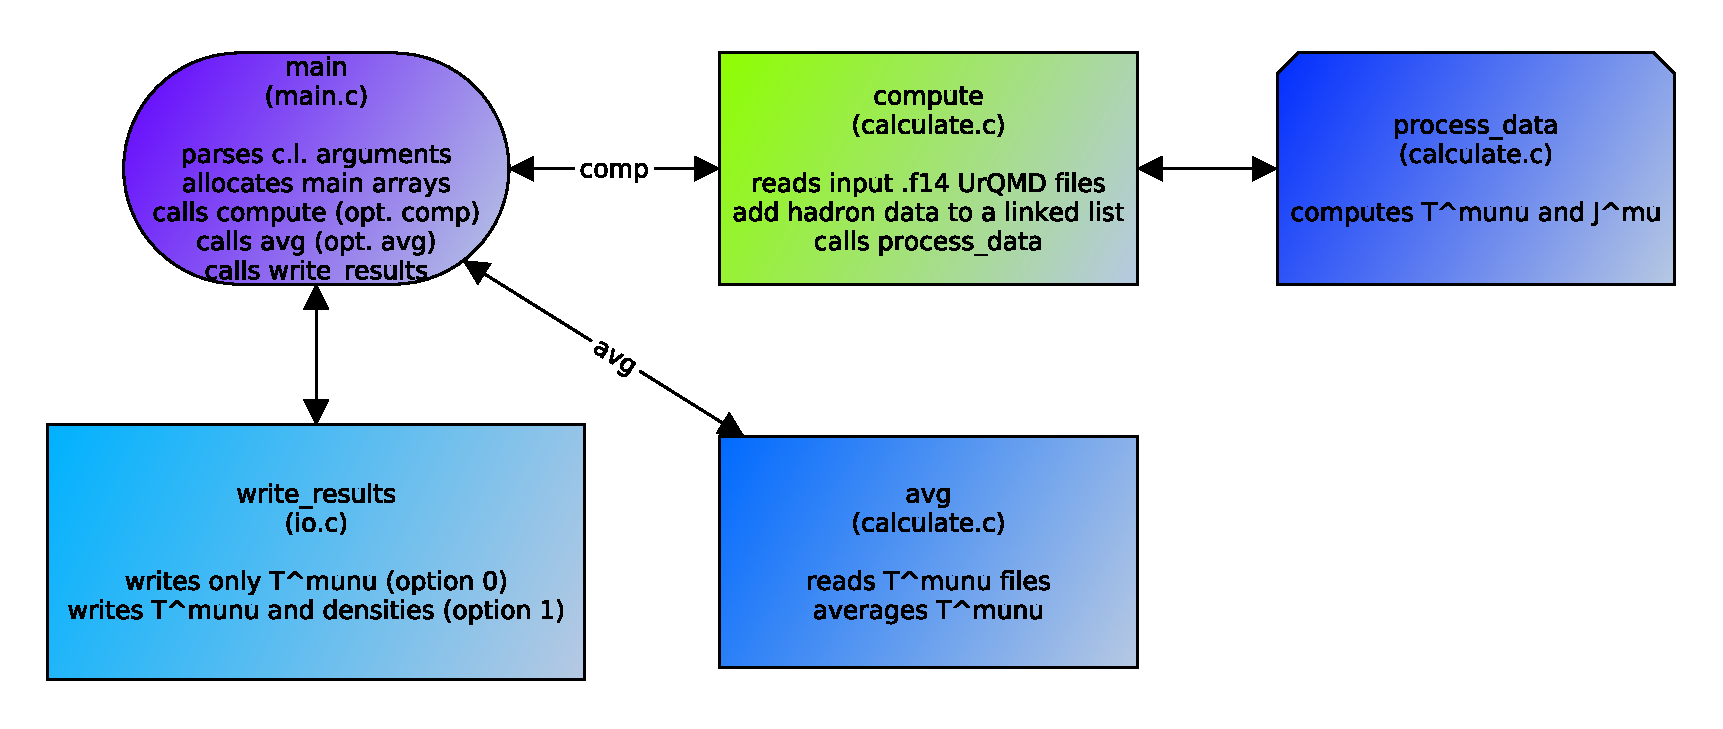
\includegraphics[width=\linewidth]{img/flow.eps}
	\caption{Structure of the main c program}
	\label{fig:workflow}
\end{figure}
The program parses the command line arguments and it allocates the most important arrays. Then, it either processes the output data of new hadronic transport simulations or it averages already existing data from previous runs, afterwards printing the results, which can optionally include the densities and the diffusion currents in the fluid LRF. The format of the output files is described in appendix \ref{app:formats}.\\
\subsection{Processing of new data}
The program reads the entries of the individual hadrons and store the data into the struct \textbf{pdata}, which contains a pointer to the next element, thus forming a list. First, the program reads all the files passed through the command line (function compute), then it processes the data. The information about the strangeness is derived on the \emph{itype} of the particle (function get\_strangeness), while the electric charge is read directly from the hadron data.\\
The energy momentum tensor and the four currents are flat 1D arrays and the elements are accessed through macros defined in \emph{definitions.h} as:
\begin{verbatim}
#define TLOC 10*(p+np*(k+nz*(j+ny*(i+(long)h*nx))))
#define JPL 4*(p+np*(k+nz*(j+ny*(i+(long)h*nx))))
#define JBL 4*(k+nz*(j+ny*(i+(long)h*nx)))
#define PNLOC (p+np*(k+nz*(j+ny*(i+(long)h*nx))))
\end{verbatim}
where \textbf{TLOC} is used for $T^{\mu\nu}$ array $Tp$, of dimension $nt\times nx \times ny \times nz \times np \times 10$, \textbf{JPL} for the four current of the hadron type $p$, stored in the array $Jp$ of dimension $nt\times nx\times ny\times nz \times np\times4$, \textbf{JBL} for the net baryon ($Jb$), strangeness ($Js$) and electric ($Jc$) conserved four currents and the non conserved total baryon + anti-baryon current ($Jt$), stored in arrays of dimension $nt \times nx \times ny \times nz \times 4$, \textbf{PNLOC} for the total number of hadron species $p$, stored in an array of dimension $nt \times nx \times ny \times nz \times np$. We recall that $nt$ is the number of timesteps, $nx$, $ny$ and $nz$ the number of cells along the x, y and z directions and $np$ is the number of ``stable'' hadrons. The number of events is stored separately and, together with the volume of the cells, it is used only at the end, when actually computing the averages by dividing the quantities in the cells by $\dd x \dd y \dd z N_{events}$.
\subsection{Averaging of old data}
This step is straightforward: we read the arrays, one file by one file, and we sum their contents, saving also the value of the new total number of events. 
\appendix
\section{Appendix}
\subsection{List of ``stable'' hadrons}\label{hadron_list}
\begin{small}
\begin{center}
	\begin{tabular}{|l | l | r | r | r | r | r |} 
		\hline
		Index & Name & B & S & e & itpye & iso3\\  
		\hline
	    1 & $\pi^-$ & 0 & 0 & -1 & 101 & -2\\
	    2 & $\pi^+$ & 0 & 0 & +1 & 101 & +2\\
	    3 & $\pi^0$ & 0 & 0 &  0 & 101 &  0\\
	    4 & $K^0$   & 0 & +1&  0 & 106 & -1\\
	    5 & $K^+$   & 0 & +1&  +1 & 106 & +1\\
	    6 & $K^-$   & 0 & -1&  -1 & -106 & -1\\
	    7 & $\bar{K}^0$ & 0 & -1&  0 & -106 & +1\\
	    8 & $N$ & 1 & 0 &  0 & +1 & -1\\
	    9 & $p$ & 1 & 0 &  +1 & +1 & +1\\
	    10 & $\bar{p}$ & -1 & 0 &  -1 & -1 & -1\\
        11 & $\bar{N}$ & -1 & 0 &  0 & -1 & +1\\
        12 & $\eta$     &  0 & 0 &  0 & 102& 0\\
        13 & $\omega$   &  0 & 0 &  0 & 103& 0\\
        14 & $\eta'$    &  0 & 0 &  0 & 107& 0\\
        15 & $\phi$     &  0 & 0 &  0 & 109& 0\\
        16 & $\Lambda_{1116}$ &  1 & -1 &  0 & 27& 0\\
        17 & $\bar{\Lambda}_{1116}$ &  -1 & +1 &  0 & -27& 0\\
        18 & $\Sigma_{1192}^-$ &  1 & -1 &  -1 & 40& -2\\
        19 & $\Sigma_{1192}^+$ &  1 & -1 &  +1 & 40& +2\\
        20 & $\Sigma_{1192}$   &  1 & -1 &   0 & 40&  0\\
        21 & $\bar{\Sigma}_{1192}^-$  &  -1 & +1 &  -1 & -40&  -2\\
        22 & $\bar{\Sigma}_{1192}^+$  &  -1 & +1 &  +1 & -40&  +2\\
        23 & $\bar{\Sigma}_{1192}$  &  -1 & +1 &  0 & -40&  0\\
        24 & $\Xi_{1317}^-$  &  1 & -2 &  -1 & 49&  -1\\
        25 & $\Xi_{1317}^0$  &  1 & -2 &   0 & 49&  +1\\
        26 & $\bar{\Xi}_{1317}^0$  &  -1 & +2 &   0 & -49&  -1\\
        27 & $\bar{\Xi}_{1317}^+$  &  -1 & +2 &  +1 & -49&   1\\
        28 & $\Lambda_{1520}$  &  1 & -2 &  0 & 29&   0\\
        29 & $\bar{\Lambda}_{1520}$  &  -1 & +2 &  0 & -29&   0\\
        30 & $\Xi_{1530}^-$  &  1 & -2 &  -1 & 50&  -1\\
        31 & $\Xi_{1520}^0$  &  1 & -2 &   0 & 50&  +1\\
        32 & $\bar{\Xi}_{1530}^0$  &  -1 & +2 &   0 & -50&  -1\\
        33 & $\bar{\Xi}_{1530}^+$  &  -1 & +2 &  +1 & -50&   1\\
        34 & $\Omega_{1672}$  &  1 & -3 &  -1 & 55&   0\\
        35 & $\bar{\Omega}_{1672}$  &  -1 & +3 &  +1 & -55&   0\\
	    
	    \hline
	 	 
	\end{tabular}
\end{center}
\end{small}
Please, note that in the code we start counting the array indexes from 0, therefore all the indexes are shifted by one position.

\subsection{Explicit form of some equations}
\subsubsection{Mixed indexes energy momentum tensor} \label{mixed_Tmunu}
It is known that $T^{\mu}_{\nu}=g_{\nu\alpha}T^{\mu\alpha}$. If $g_{\nu\alpha}=g^{\nu\alpha}=diag(1,-1,-1,-1)$ is the Minkowski metric tensor with ``West Coast'' signature, then:
\begin{equation}
\begin{split}
T^0_0=g_{00}T^{00}+\cancel{g_{01}T^{01}}+\cancel{g_{02}T^{02}}+\cancel{g_{03}T^{03}}=T^{00},\\
T^0_1=\cancel{g_{10}T^{00}}+g_{11}T^{01}+\cancel{g_{12}T^{02}}+\cancel{g_{13}T^{03}}=-T^{01}=-T^{10},\\
T^0_2=\cancel{g_{20}T^{00}}+\cancel{g_{21}T^{01}}+g_{22}T^{02}+\cancel{g_{23}T^{03}}=-T^{02}=-T^{20},\\
T^0_3=\cancel{g_{30}T^{00}}+\cancel{g_{31}T^{01}}+\cancel{g_{32}T^{02}}+g_{33}T^{03}=-T^{03}=-T^{30},\\
T^1_0=g_{00}T^{10}+\cancel{g_{01}T^{11}}+\cancel{g_{02}T^{12}}+\cancel{g_{03}T^{13}}=T^{10}=T^{01},\\
T^1_1=\cancel{g_{10}T^{10}}+g_{11}T^{11}+\cancel{g_{12}T^{12}}+\cancel{g_{13}T^{13}}=-T^{11},\\
T^1_2=\cancel{g_{20}T^{10}}+\cancel{g_{21}T^{11}}+g_{22}T^{12}+\cancel{g_{23}T^{13}}=-T^{12}=-T^{21},\\
T^1_3=\cancel{g_{30}T^{10}}+\cancel{g_{31}T^{11}}+\cancel{g_{32}T^{12}}+g_{33}T^{13}=-T^{13}=-T^{31},\\
T^2_0=g_{00}T^{20}+\cancel{g_{01}T^{21}}+\cancel{g_{02}T^{22}}+\cancel{g_{03}T^{23}}=T^{20}=T^{02},\\
T^2_1=\cancel{g_{10}T^{20}}+g_{11}T^{21}+\cancel{g_{12}T^{22}}+\cancel{g_{13}T^{23}}=-T^{21}=-T^{12},\\
T^2_2=\cancel{g_{20}T^{20}}+\cancel{g_{21}T^{21}}+g_{22}T^{22}+\cancel{g_{23}T^{23}}=-T^{22},\\
T^2_3=\cancel{g_{30}T^{20}}+\cancel{g_{31}T^{21}}+\cancel{g_{32}T^{22}}+g_{33}T^{23}=-T^{23}=-T^{32},\\
T^3_0=g_{00}T^{30}+\cancel{g_{01}T^{31}}+\cancel{g_{02}T^{32}}+\cancel{g_{03}T^{33}}=T^{30}=T^{03},\\
T^3_1=\cancel{g_{10}T^{30}}+g_{11}T^{31}+\cancel{g_{12}T^{32}}+\cancel{g_{13}T^{33}}=-T^{31}=-T^{13},\\
T^3_2=\cancel{g_{20}T^{30}}+\cancel{g_{21}T^{31}}+g_{22}T^{32}+\cancel{g_{23}T^{33}}=-T^{32}=-T^{23},\\
T^3_3=\cancel{g_{30}T^{30}}+\cancel{g_{31}T^{31}}+\cancel{g_{32}T^{32}}+g_{33}T^{33}=-T^{33}.
\end{split}
\end{equation}
So, finally we get:
\begin{equation}
T^{\mu}_{\nu}=
\begin{pmatrix}
T^{00}&-T^{01}&-T^{02}&-T^{03}\\
T^{10}&-T^{11}&-T^{12}&-T^{13}\\
T^{20}&-T^{21}&-T^{22}&-T^{23}\\
T^{30}&-T^{31}&-T^{32}&-T^{33}\\
\end{pmatrix}.
\label{mixed_Tmunu_matrix}
\end{equation}
\subsection{Format of the output files}\label{app:formats}
\subsubsection{Energy-momentum tensor files}
The files containing the energy-momentum tensors and the four-currents produced by the main program have the following structure: a preamble containing the basic information about the grid and then a sequence of multi-dimensional arrays.\\

\begin{minipage}{0.6\textwidth}
	\centering
	\begin{tabular}{|c | c |} 
		\hline
		\cellcolor{Yellow}Variable & \cellcolor{Yellow} C type \\
		\hline
		\cellcolor{SpringGreen}number of events&\cellcolor{SpringGreen}long int\\
		\hline
		\cellcolor{LimeGreen}time&\cellcolor{LimeGreen}double\\
		\hline
		\cellcolor{YellowGreen}number of hadrons np&\cellcolor{YellowGreen}int\\
		\hline
		\cellcolor{SeaGreen}numb. of x cells nx&\cellcolor{SeaGreen}int\\
		\hline
		\cellcolor{SeaGreen}numb. of y cells ny&\cellcolor{SeaGreen}int\\
		\hline
		\cellcolor{SeaGreen}numb. of z cells nz&\cellcolor{SeaGreen}int\\
		\hline
		\cellcolor{BlueGreen}dx&\cellcolor{BlueGreen}double\\
		\hline
		\cellcolor{BlueGreen}dy&\cellcolor{BlueGreen}double\\
		\hline
		\cellcolor{BlueGreen}dz&\cellcolor{BlueGreen}double\\
		\hline
	\end{tabular}\\
	\vspace{1mm}
	\footnotesize{Data at the beginning of each file}
	\vspace{5mm}	
\end{minipage}
\begin{minipage}{0.4\textwidth}
	\centering
	\begin{tabular}{| c | c |} 
		\hline
		\cellcolor{Yellow}Array & \cellcolor{Yellow} Dimensions \\
		\hline
		\cellcolor{SpringGreen}$T_p$&\cellcolor{SpringGreen}nx$\times$ny$\times$nz$\times$np$\times$10\\
		\hline
		\cellcolor{LimeGreen}$J_p$&\cellcolor{LimeGreen}nx$\times$ny$\times$nz$\times$np$\times$4\\
		\hline
		\cellcolor{ForestGreen}$J_b$&\cellcolor{ForestGreen}nx$\times$ny$\times$nz$\times$4\\
		\hline
		\cellcolor{SkyBlue}$J_c$&\cellcolor{SkyBlue}nx$\times$ny$\times$nz$\times$4\\
		\hline
		\cellcolor{Turquoise}$J_s$&\cellcolor{Turquoise}nx$\times$ny$\times$nz$\times$4\\
		\hline
		\cellcolor{Cerulean}$J_t$&\cellcolor{Cerulean}nx$\times$ny$\times$nz$\times$4\\
		\hline
		\cellcolor{RoyalBlue}Pnum&\cellcolor{RoyalBlue}nx$\times$ny$\times$nz$\times$np\\
		\hline
	\end{tabular}\\
	\vspace{1mm}
	\footnotesize{Sequence of the arrays.}
\end{minipage}

We recall that the first index (x) is the slowest. We also recall that: $T_p$ and $J_p$ are the multidimensional arrays containing the energy-momentum tensors and the four currents, respectively, of the individual hadron species, $J_b$ is the net baryon four current, $J_c$ the net electric charge four current, $J_s$ the strangeness four current, $J_t$ the total baryon and anti-baryon four current (not conserved), Pnum the number of hadrons of the various species in each cell, np, the number of evaluated ``stable'' hadron species is equal to NP (set in \emph{definitions.h}) plus 1 additional ``catch-all'' entry for unidentified hadrons. The C data type of the multidimensional arrays is double. In the four currents, the index 0 refers to time, index 1 to x, index 2 to y and index 3 to z. In the energy momentum tensors (which are symmetric): $0=T^{00}$, $1=T^{01}$, $2=T^{02}$, $3=T^{03}$, $4=T^{11}$, $5=T^{12}$, $6=T^{13}$, $7=T^{22}$, $8=T^{23}$, $9=T^{33}$. 

\subsubsection{Density files}
The ``density'' files produced by the main program have the following structure: a preamble containing the basic information about the grid and then, for each point of the grid, the densities.\\

\begin{minipage}{0.6\textwidth}
	\centering
	\begin{tabular}{|c | c |} 
		\hline
		\cellcolor{Yellow}Variable & \cellcolor{Yellow} C type \\
		\hline
		\cellcolor{SpringGreen}number of events&\cellcolor{SpringGreen}long int\\
		\hline
		\cellcolor{LimeGreen}time&\cellcolor{LimeGreen}double\\
		\hline
		\cellcolor{YellowGreen}number of hadrons np&\cellcolor{YellowGreen}int\\
		\hline
		\cellcolor{SeaGreen}numb. of x cells nx&\cellcolor{SeaGreen}int\\
		\hline
		\cellcolor{SeaGreen}numb. of y cells ny&\cellcolor{SeaGreen}int\\
		\hline
		\cellcolor{SeaGreen}numb. of z cells nz&\cellcolor{SeaGreen}int\\
		\hline
		\cellcolor{BlueGreen}dx&\cellcolor{BlueGreen}double\\
		\hline
		\cellcolor{BlueGreen}dy&\cellcolor{BlueGreen}double\\
		\hline
		\cellcolor{BlueGreen}dz&\cellcolor{BlueGreen}double\\
		\hline
	\end{tabular}\\
    \vspace{1mm}
    \footnotesize{Data at the beginning of each file}

\end{minipage}
\begin{minipage}{0.4\textwidth}
	\centering
	\begin{tabular}{|l | c |} 
		\hline
		\cellcolor{Yellow}Index & \cellcolor{Yellow} Quantity \\
		\hline
		\cellcolor{SpringGreen}0&\cellcolor{SpringGreen}$\rho_{\mathrm{B}}$\\
		\hline
		\cellcolor{LimeGreen}1&\cellcolor{LimeGreen}$v_x(n_{\mathrm{B}})$\\
		\hline
		\cellcolor{LimeGreen}2&\cellcolor{LimeGreen}$v_y(n_{\mathrm{B}})$\\
		\hline
		\cellcolor{LimeGreen}3&\cellcolor{LimeGreen}$v_z(n_{\mathrm{B}})$\\
		\hline
		\cellcolor{ForestGreen}4&\cellcolor{ForestGreen}$\rho_{\mathrm{B}+\mathrm{\bar{B}}}$\\
		\hline
		\cellcolor{SkyBlue}5&\cellcolor{SkyBlue}$\rho_{\mathrm{C}}$\\
		\hline
		\cellcolor{Turquoise}6&\cellcolor{Turquoise}$\rho_{\mathrm{S}}$\\
		\hline
		\cellcolor{Cerulean}7&\cellcolor{Cerulean}$I^0_{\mathrm{C}}$\\
		\hline
		\cellcolor{Cerulean}8&\cellcolor{Cerulean}$I^1_{\mathrm{C}}$\\
		\hline
		\cellcolor{Cerulean}9&\cellcolor{Cerulean}$I^2_{\mathrm{C}}$\\
		\hline
		\cellcolor{Cerulean}10&\cellcolor{Cerulean}$I^3_{\mathrm{C}}$\\
		\hline
		\cellcolor{Orchid}11&\cellcolor{Orchid}$I^0_{\mathrm{S}}$\\
		\hline
		\cellcolor{Orchid}12&\cellcolor{Orchid}$I^1_{\mathrm{S}}$\\
		\hline
		\cellcolor{Orchid}13&\cellcolor{Orchid}$I^2_{\mathrm{S}}$\\
		\hline
		\cellcolor{Orchid}14&\cellcolor{Orchid}$I^3_{\mathrm{S}}$\\
		\hline
		\cellcolor{Yellow}&\cellcolor{Yellow}$\forall$ hadron p, 0$<$p$<$np-1\\
		\cellcolor{Lavender}15+3$\cdot$p&\cellcolor{Lavender}num. of hadrons p\\
		\hline
		\cellcolor{Lavender}16+3$\cdot$p&\cellcolor{Lavender}$\rho_p$\\
		\hline
		\cellcolor{Lavender}17+3$\cdot$p&\cellcolor{Lavender}$\varepsilon_p$\\
		\hline		
	\end{tabular}\\
\vspace{1mm}
    \footnotesize{Data for each point of the grid.\\C type: double for all entries.}
    \vspace{5mm}
  \end{minipage}

We recall that the number of hadrons is NP+1, where NP is the value written in \emph{definitions.h}, because the code automatically adds an entry for the unidentified hadrons.\\
We also recall that the fastest index is z, then y, then x.\\


\subsection{Known issues and possible improvements}
\subsubsection{Issues}
\begin{itemize}
	\item combining the results at different timesteps can be quite tricky
	\item the control of the memory usage is quite raw
\end{itemize}

\subsubsection{Possible improvements}
\begin{itemize}
	\item we might consider to use dynamical multi-dimensional arrays instead of a big single-array. Cons: more tricky to implement, maybe slightly slower. Pro: code easier to read, memory usage more efficient.
	\item we might consider to use MPI	
\end{itemize}

\subsection{Common settings of UrQMD simulations}
Here we briefly review the key parameters to set up the UrQMD simulations to prepare the hadron data to be processed by the coarse graining code.\\
This short review is far from being complete. For a comprehensive description of the various options, please, refer to the UrQMD manual.\\
Regarding specifically the coarse-graining approach, in general the most important parameters are:\\

\begin{verbatim}
pro 197 79
tar 197 79
\end{verbatim}
Here we choose the target and the projectile, in this case gold in both cases.\\

\begin{verbatim}
imp -3.4
\end{verbatim}

The impact parameter b in fm. In this case we use b ranging from 0 to 3.4 fm.\\

\begin{verbatim}
nev 1500
\end{verbatim}
The number of events. Since the number of produced particles grows with the collision energy, the output .f14 files grows in size, as well. To prevent the creation of very large files, which might be more difficult to handle, sometimes it is better to run more UrQMD simulations with less events than just a few UrQMD simulations with a lot of events each.\\

\begin{verbatim}
rsd 5016522
\end{verbatim}
This is the integer number to initialize the random number generator. It should be changed each time we run UrQMD. Usually it is convenient to change it by preliminary using a script.\\

\begin{verbatim}
ecm 7.7
\end{verbatim}
The collision energy in GeV/nucleaon (please, remember to use elb instead of ecm for the beam energy in fixed target experiments).\\

\begin{verbatim}
tim 80 0.5
\end{verbatim}
The first number fixes the final time of the simulations and the second number the timestep, which will be also the resolution of the coarse graining evolution. Of course the total number of timesteps will be the ratio between the first and the second number.
If we want to use the coarse graining data to assign a temperature and a chemical potential to an external list of particle, it is recommended first to study the time distribution of this list of particle data and then choose tim appropriately.

\begin{verbatim}
f13
\#f14
f15
f16
f19
f20
\end{verbatim}
Usually, instead of manually set up the configuration files, it is convenient to write a bash script that automatically takes care of that, especially if we use a computer cluster.
In the following section we provide an example for the CSC Goethe cluster in Frankfurt am Main.

\bibliography{bibliography.bib}
\bibliographystyle{ieeetr}

\end{document}
